\documentclass[a4paper,12pt]{article}
\setlength{\headheight}{68.803pt}
\addtolength{\topmargin}{-56.803pt}

\usepackage[utf8]{inputenc}
\usepackage[T1]{fontenc}
\usepackage{lmodern}
\usepackage[nopatch=footnote]{microtype}
\usepackage{fvextra}
\DefineVerbatimEnvironment{Verbatim}{Verbatim}{
  breaklines=true,
  breakanywhere=true,
  frame=single,
  fontsize=\small
}

% margin settings
\usepackage[
  left=1in,
  right=1in,
  top=3cm,
  bottom=1in
]{geometry}

\usepackage[
    colorlinks=true,
    linkcolor=black,
    urlcolor=blue,
    citecolor=blue,
    pdfborder={0 0 0},
    pdfauthor={Massimo Mantineo},
    pdftitle={Client Multicast UDP},
    pdfsubject={Laboratorio di Reti e Sistemi Distribuiti: HANDS-ON 6},
]{hyperref}

\usepackage{graphicx}
\graphicspath{{../../assets/}{../../assets/ho1/}{../../assets/ho2/}{../../assets/ho3/}{../../assets/ho4/}{../../assets/ho5/}{../../assets/ho6/}{../../assets/ho7/}{../../assets/ho8/}{../../assets/ho10/}}
\usepackage{tikz}
\usetikzlibrary{positioning, arrows.meta}
\usepackage{listings}
\usepackage{xcolor}
\usepackage{amsmath, amssymb}
\usepackage{fancyhdr}
\usepackage{setspace}
\usepackage{pgfplots}
\pgfplotsset{compat=1.17}
\usepackage{booktabs}
\usepackage[skins, listings]{tcolorbox}
\usepackage{float}

\newtcblisting{terminal}[1][]{
    listing only,
    colback=black!85!white,
    colframe=black!70!white,
    colupper=green!80!white,
    coltitle=white,
    title=#1,
    fonttitle=\bfseries\sffamily,
    listing options={
        language={},
        basicstyle=\ttfamily\small\color{green!80!white},
        backgroundcolor={},
        frame=none,
        breaklines=true,
        showstringspaces=false,
        numbers=none
    },
    enhanced,
    drop shadow,
    arc=3mm
}

\newtcblisting{ccode}[1][]{
    listing only,
    colback=blue!3!white,
    colframe=blue!70!black,
    title=#1,
    fonttitle=\bfseries\sffamily,
    listing options={
        style=cstyle,
        backgroundcolor={},
        frame=none
    },
    enhanced,
    drop shadow,
    arc=3mm
}

\setlength{\footskip}{50pt}

% settings for C listings
\lstdefinestyle{cstyle}{
    language=C,
    basicstyle=\ttfamily\small,
    numbers=left,
    numberstyle=\tiny,
    stepnumber=1,
    numbersep=5pt,
    backgroundcolor=\color{white},
    showspaces=false,
    showstringspaces=false,
    showtabs=false,
    frame=single,
    tabsize=4,
    captionpos=b,
    breaklines=true,
    breakatwhitespace=true,
    keywordstyle=\color{blue}\bfseries,
    commentstyle=\color{green!50!black},
    stringstyle=\color{red},
}
\lstset{style=cstyle}

% Header and Footer
\pagestyle{fancy}
\fancyhf{}

\fancyhead[L]{%
  \parbox[b]{0.45\textwidth}{%
    \small
    Student Name: Massimo Mantineo\\
    Student ID: 541924
    \vspace{20pt}
  }%
}
\fancyhead[C]{%
  \parbox[b]{0.2\textwidth}{%
    \centering
    \normalsize \bfseries
    LabReSiD25\\
    Hands-On 6
    \vspace{20pt}
  }%
}
\fancyhead[R]{%
  \parbox[b]{0.35\textwidth}{%
    \flushright
    
\includegraphics[width=3.5cm]{logo_unime_orizontale.png}
    \vspace{15pt}
  }%
}

\renewcommand{\contentsname}{Indice}

\title{\vspace{-2cm}Report: Client UDP Multicast\\
\large (Hands-On 6)}
\author{Massimo Mantineo \\ Matricola: 541924}
\date{MESSINA, A.A. 2024/2025}

\begin{document}

% Cover page
\begin{titlepage}
    \thispagestyle{empty}
    \centering
    \vspace*{1cm}
    
\includegraphics[width=6cm]{logo_unime_orizontale.png}\par\vspace{1cm}
    \vspace{2cm}
    {\Large \textbf{Università degli Studi di Messina}\par}
    {\large Dipartimento MIFT - Corso di Laurea Triennale in Informatica (L-31)\par}
    \vspace*{1cm}
    {\large Laboratorio di Reti e Sistemi Distribuiti\par}
    \vspace{1cm}
    {\Large \textbf{HANDS-ON 6:}\\
    Client UDP Multicast\par}
    \vspace{2cm}
    {\large Massimo Mantineo \par}
    {\large Matricola: 541924 \par}
    \vfill
    {\large Messina, A.A. 2024/2025 \par}
\end{titlepage}

\clearpage
\pagestyle{fancy}
\tableofcontents
\newpage

\section{Problem Statement}
L'obiettivo della sesta esercitazione (Hands-On 6) è lo sviluppo di un client UDP multicast in linguaggio C. Il client deve potersi unire a un gruppo multicast al fine di ricevere i messaggi del server fornito dal Docente (\texttt{multicast\_server.c}). Viene richiesto inoltre che sia possibile lanciare molteplici istanze del client in parallelo per ricevere i messaggi simultaneamente.

\section{Stato dell'Arte}
La comunicazione multicast è di tipo uno-a-molti: un host invia un messaggio una singola volta e la rete, utilizzando protocolli come all'IGMP (Internet Group Management Protocol), si assicura di replicarlo e recapitarlo a tutti gli host iscritti.

A livello di sistema (socket API), la gestione del multicast avviene tramite una serie di direttive con cui il processo informa il kernel della propria volontà di inoltrare la sottoscrizione al gruppo. Le procedure implementate sono le seguenti:


\section{Metodologia ed Implementazione}

Il codice sorgente per il multicast si basa su due strutture principali e sull'uso mirato di \texttt{setsockopt()}.

\begin{ccode}[1 e 2: Creazione Socket e SO\_REUSEADDR]
int sockfd;
if ((sockfd = socket(AF_INET, SOCK_DGRAM, 0)) < 0) {
    perror("Socket creation failed");
    exit(EXIT_FAILURE);
}

int reuse = 1;
if (setsockopt(sockfd, SOL_SOCKET, SO_REUSEADDR, &reuse, sizeof(reuse)) < 0) {
    perror("SO_REUSEADDR failed");
    exit(EXIT_FAILURE);
}
\end{ccode}

Si effettua quindi il bind e si provvede all'iscrizione al gruppo Multicast (nel nostro caso \texttt{239.0.0.1}).
\begin{ccode}[3 e 4: Bind e Add Membership]
// Bind
local_addr.sin_family = AF_INET;
local_addr.sin_port = htons(PORT);
local_addr.sin_addr.s_addr = INADDR_ANY;
bind(sockfd, (struct sockaddr *)&local_addr, sizeof(local_addr));

// Iscrizione Multicast
struct ip_mreq multicast_req;
multicast_req.imr_multiaddr.s_addr = inet_addr("239.0.0.1");
multicast_req.imr_interface.s_addr = INADDR_ANY;

setsockopt(sockfd, IPPROTO_IP, IP_ADD_MEMBERSHIP, &multicast_req, sizeof(multicast_req));
\end{ccode}

\newpage
Nel loop principale si esegue in ultimo la normale \texttt{recvfrom()} bloccante per ricevere il payload su pacchetti inviati in UDP.
\begin{ccode}[5: Ricezione dei messaggi UDP]
while (1) {
    int n = recvfrom(sockfd, buffer, MAX_BUFFER - 1, 0, 
                     (struct sockaddr *)&sender_addr, &sender_len);
    // ... logic per stampa e gestione terminazione ...
}

// 6: Dropout in dismissione
setsockopt(sockfd, IPPROTO_IP, IP_DROP_MEMBERSHIP, &multicast_req, sizeof(multicast_req));
\end{ccode}


\subsection{Istruzioni di Esecuzione}
Compilazione della suite multicast:
\begin{terminal}[Multicast Build]
$ gcc multicast_server.c -o server
$ gcc multicast_client.c -o client
\end{terminal}

\section{Risultati}
Per validare il comportamento del software, sono stati testati esecutivamente due processi client separati ed un unico mittente (il server multicast) sulla medesima subnet.

\subsection{Istanziare molteplici Client}
I log di terminale sottostanti dimostrano come il kernel riceva il traffico multicast unificato, recapitando lo stream del buffer "Hello, Multicast!" ad ogni terminale.

\begin{terminal}[Terminale 1 - Server]
$ ./server
Sent: Hello, Multicast!
Sent: Hello, Multicast!
Sent: Hello, Multicast!
\end{terminal}

\begin{terminal}[Terminale 2 - Client 1]
$ ./client
Client iscritto al gruppo multicast 239.0.0.1 sulla porta 12345
In attesa di messaggi...

Ricevuto: Hello, Multicast! | (Da: 127.0.0.1:46155)
Ricevuto: Hello, Multicast! | (Da: 127.0.0.1:46155)
\end{terminal}

\begin{terminal}[Terminale 3 - Client 2]
$ ./client
Client iscritto al gruppo multicast 239.0.0.1 sulla porta 12345
In attesa di messaggi...

Ricevuto: Hello, Multicast! | (Da: 127.0.0.1:46155)
Ricevuto: Hello, Multicast! | (Da: 127.0.0.1:46155)
\end{terminal}

Entrambi i socket UDP sono stati abilitati alla convivenza sullo stesso port listening e intercettano con precisione i messaggi mandati in overlay sull'IP appartenente al gruppo di classe D.

\subsection{Analisi Wireshark}
L'analisi del traffico tramite Wireshark (Figura \ref{fig:wireshark_multicast}) conferma il corretto inoltro dei pacchetti UDP verso l'indirizzo di classe D \texttt{239.0.0.1}. Si osserva come un singolo pacchetto inviato dal server venga ricevuto da tutti i client iscritti al gruppo, minimizzando il carico di rete rispetto ad una comunicazione unicast multipla.

\begin{figure}[H]
    \centering
    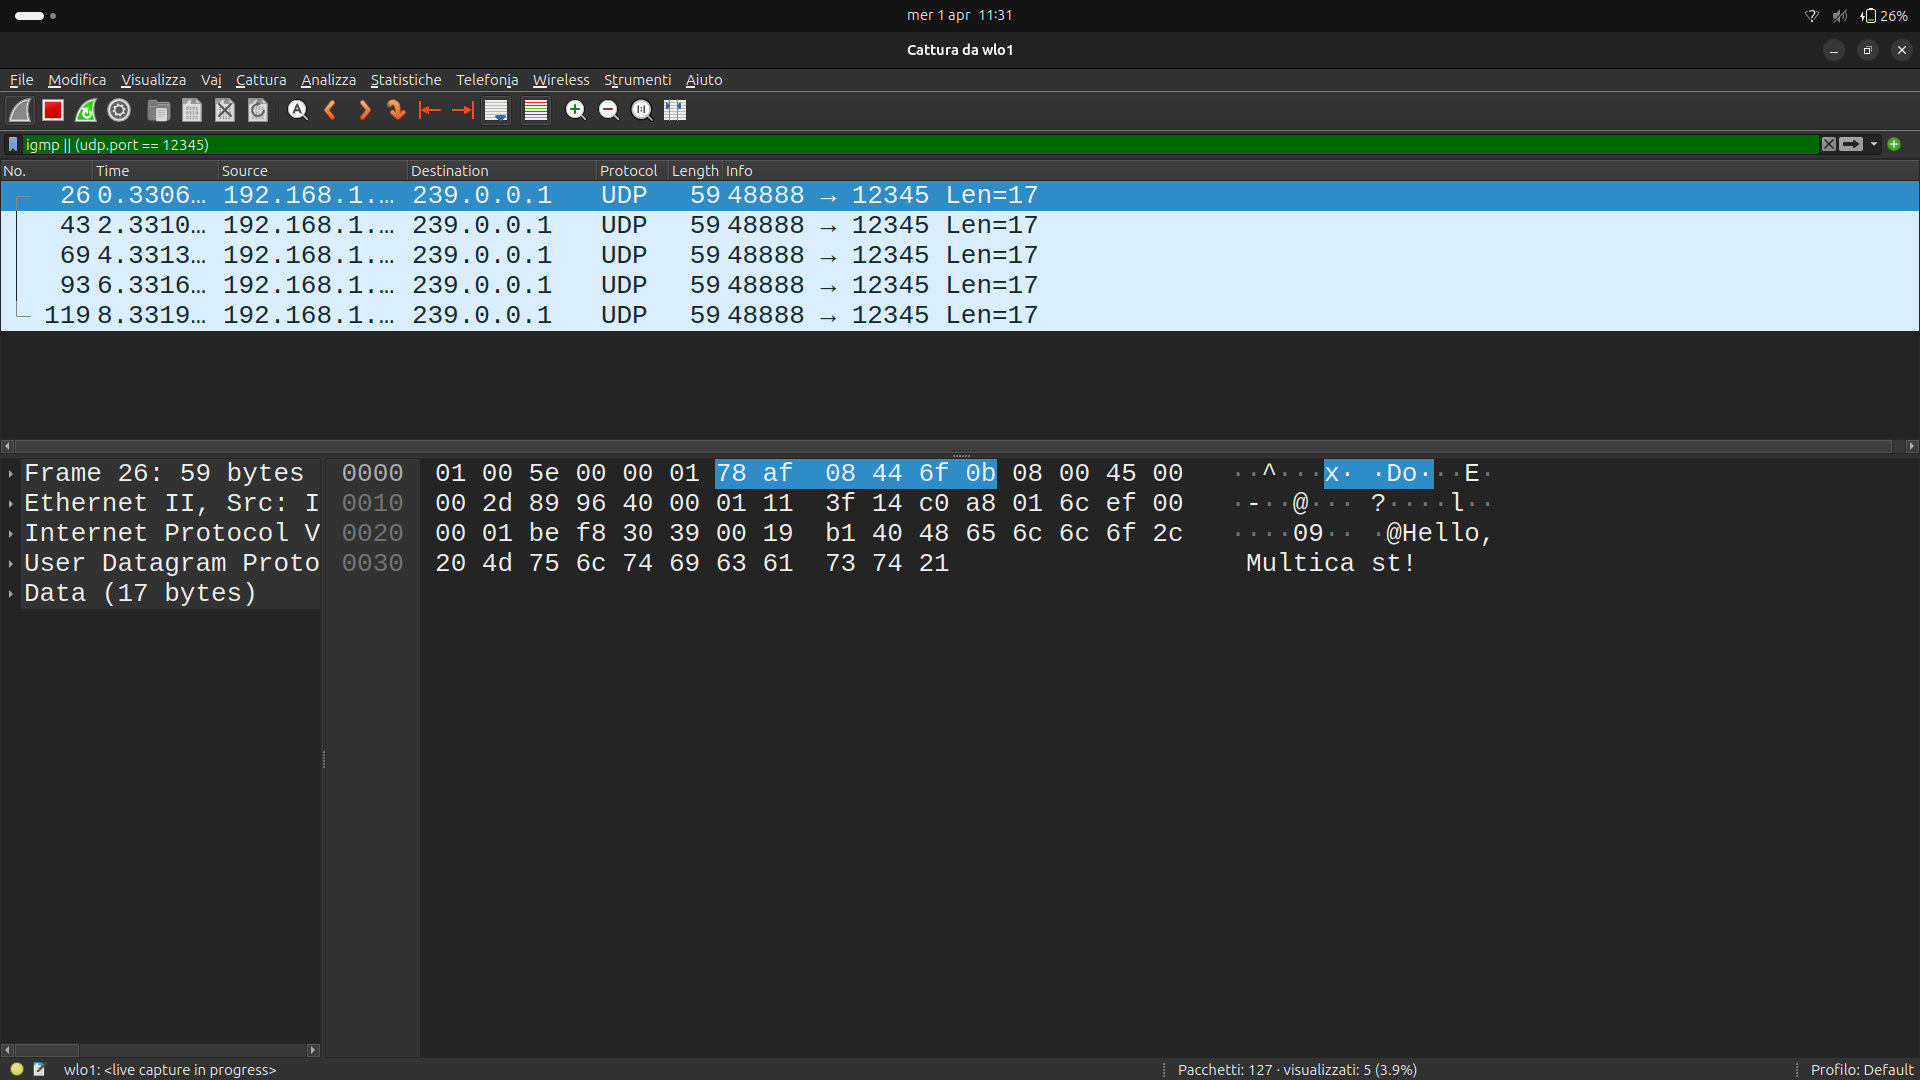
\includegraphics[width=0.9\textwidth]{ho6_wireshark_multicast.png}
    \caption{Cattura Wireshark: Flusso Multicast UDP verso 239.0.0.1}
    \label{fig:wireshark_multicast}
\end{figure}

\section{Conclusioni e Sviluppi Futuri}
Durante l'Hands-On 6 è stato analizzato l'assetto implementativo richiesto per abilitare flussi uno-a-molti nelle architetture basate su datagrammi in linguaggio C, superando in modo efficace i vincoli stringenti dettati dall'API standard ed approfondendo i benefici dell'opzione estesa SO\_REUSEADDR e l'invio degli intent IGMP via syscall.


\begin{itemize}
    \item \textbf{Analisi Prestazionale}: Studio dell\'impatto della latenza di sistema sulla scalabilità dell\'architettura.
    \item \textbf{Ottimizzazione delle Risorse}: Refactoring del codice per minimizzare l\'uso della CPU in contesti ad alta concorrenza.
\end{itemize}
\end{document}